%%%%%%%%%%%%%%%%%%%%%%%%%%%%%%%%%%%%%%%%%
% Jacobs Landscape Poster
% LaTeX Template
% Version 1.0 (29/03/13)
%
% Created by: 
% Computational Physics and Biophysics Group, Jacobs University
% https://teamwork.jacobs-university.de:8443/confluence/display/CoPandBiG/LaTeX+Poster
% 
% Further modified by:
% Nathaniel Johnston (nathaniel@njohnston.ca)
%
% This template has been downloaded from:
% http://www.LaTeXTemplates.com
%
% License:
% CC BY-NC-SA 3.0 (http://creativecommons.org/licenses/by-nc-sa/3.0/)
%
%%%%%%%%%%%%%%%%%%%%%%%%%%%%%%%%%%%%%%%%%

%----------------------------------------------------------------------------------------
%	PACKAGES AND OTHER DOCUMENT CONFIGURATIONS
%----------------------------------------------------------------------------------------

\documentclass[final]{beamer}

\usepackage[scale=1.24]{beamerposter} % Use the beamerposter package for laying out the poster

% \usepackage[scale=1.24]{beamerposter} % Use the beamerposter package for laying out the poster

\usetheme{confposter} % Use the confposter theme supplied with this template

\usepackage{xcolor} % Adding custom colors like SFU red
% https://www.sfu.ca/clf/colour-palette.html

\definecolor{ultramarine}{RGB}{0,32,96}

\definecolor{sfured}{RGB}{166,25,46}

\definecolor{sfublack}{RGB}{84,88,90}

\definecolor{sfumaroon}{RGB}{84,25,34}

\setbeamercolor{block title}{fg=sfumaroon,bg=white} % Colors of the block titles
\setbeamercolor{block body}{fg=black,bg=white} % Colors of the body of blocks
\setbeamercolor{block alerted title}{fg=white,bg=sfured!70} % Colors of the highlighted block titles
\setbeamercolor{block alerted body}{fg=black,bg=sfured!10} % Colors of the body of highlighted blocks
% Many more colors are available for use in beamerthemeconfposter.sty

%-----------------------------------------------------------
% Define the column widths and overall poster size
% To set effective sepwid, onecolwid and twocolwid values, first choose how many columns you want and how much separation you want between columns
% In this template, the separation width chosen is 0.024 of the paper width and a 4-column layout
% onecolwid should therefore be (1-(# of columns+1)*sepwid)/# of columns e.g. (1-(4+1)*0.024)/4 = 0.22
% Set twocolwid to be (2*onecolwid)+sepwid = 0.464
% Set threecolwid to be (3*onecolwid)+2*sepwid = 0.708

\newlength{\sepwid}
\newlength{\onecolwid}
\newlength{\twocolwid}
\newlength{\threecolwid}
\setlength{\paperwidth}{48in} % A0 width: 46.8in
\setlength{\paperheight}{36in} % A0 height: 33.1in

% \setlength{\paperwidth}{36in} % A0 width: 46.8in
% \setlength{\paperheight}{24in} % A0 height: 33.1in

\setlength{\sepwid}{0.024\paperwidth} % Separation width (white space) between columns
% \setlength{\onecolwid}{0.22\paperwidth} % Width of one column
\setlength{\onecolwid}{0.28\paperwidth} % Width of one column
\setlength{\twocolwid}{0.464\paperwidth} % Width of two columns
\setlength{\threecolwid}{0.708\paperwidth} % Width of three columns
\setlength{\topmargin}{-0.5in} % Reduce the top margin size
%-----------------------------------------------------------

\usepackage{graphicx}  % Required for including images

\usepackage{booktabs} % Top and bottom rules for tables

\usepackage{siunitx}
\usepackage{numprint}

\usepackage{tikz} % Inserting logo
%----------------------------------------------------------------------------------------
%	TITLE SECTION 
%----------------------------------------------------------------------------------------

\title{Detecting Misstatements in Financial Statements} % Poster title

\author{Vincent Chiu, Vishal Shukla, Kanika Sanduja} % Author(s)

\institute{CS Department, Simon Fraser University} % Institution(s)

%----------------------------------------------------------------------------------------

\begin{document}

\addtobeamertemplate{headline}{} 
{
\begin{tikzpicture}[remember picture,overlay] 
\node [shift={(-10 cm,-6.5 cm)}] at (current page.north east) {
\includegraphics[height=10cm]{SFUBigData_logo.jpg}}; 
\end{tikzpicture} 
}

\addtobeamertemplate{block end}{}{\vspace*{2ex}} % White space under blocks
\addtobeamertemplate{block alerted end}{}{\vspace*{2ex}} % White space under highlighted (alert) blocks

\setlength{\belowcaptionskip}{2ex} % White space under figures
\setlength\belowdisplayshortskip{2ex} % White space under equations

\begin{frame}[t] % The whole poster is enclosed in one beamer frame

\begin{columns}[t] % The whole poster consists of three major columns, the second of which is split into two columns twice - the [t] option aligns each column's content to the top

\begin{column}{\sepwid}\end{column} % Empty spacer column

\begin{column}{\onecolwid} % The first column

\begin{block}{Motivation and Background} 
\begin{itemize}
% \item Help society invest with confidence
% \item Corporations will be more responsible
\item Enable auditors to focus on companies that are more likely to make a misstatement. 
\item Investors will be able take into account the misstatement risk in their decisions. 
\end{itemize}
\end{block}

\begin{alertblock}{Problem Statement} 
% What questions do you want to answer? 
\begin{itemize}
\item Is it possible to detect whether or not a given financial report has been misstated?
% \item How correlated are the fields of a financial statement?
\item Which industry has the most misstatements?
% \item What are the most common reasons for misstatements?

% Is it possible to use unsupervised learning to identify corporations that are outliers?
% Is there a correlation between a corporation being an outlier and submitting misstated financial
% reports?
\end{itemize}

Why are they challenging?\\
\begin{itemize}
\item Very large data set with hundreds of thousands of financial statements
\item integrating multiple data sets
% \item Only have the restated financial data available, all misstated data has already been corrected.
\item Very few examples of actual misstated financial statements. 
% \item The majority of features contain mostly null values
\item having to acquire accounting domain knowledge
\end{itemize}
\end{alertblock}

\begin{block}{Data Science Pipeline} 

% What's your data-science pipeline like? Describe each component in detail.
\begin{itemize}
\item CompuStat annual report data: 1000s of corporations, around 500,000 financial statements
\item Accounting and Auditing Enforcement Releases (AAER) data: data representing companies found guilty of misstatements. We used this as our training label.
\item IBES analyst earnings per share prediction data:
\item Data Integration, joining tables through stock ticker and report year.
% to be filled out by Vishal here
\end{itemize}
\end{block}



\begin{block}{Methodology} 
% What tools or analysis methods did you use? Why did you choose them? How did you apply them to tackling each problem
Preprocessing: We took the integrated dataset and imputed zeros in place of the null values.  We only used the numerical variables.\\
Models:
\begin{itemize}
\item Random Forest: ensemble learning with multiple decision trees
\item Logistic Regression: estimating probabilities using a logistic function and applying a threshold to the probability to classify.
\item k-Means: 
\end{itemize}
Tools:
\begin{itemize}
\item For Machine Learning: Spark, Spark ML
\item For Visualization: matplotlib, Bokeh, Tableau.
\end{itemize}
\end{block}

\end{column} % End of the first column
\begin{column}{\sepwid}\end{column} % Empty spacer column
\begin{column}{\onecolwid} 

\begin{alertblock}{Evaluation} 
% Why is your solution good? Why does your result make sense?
We have a high accuracy and a fairly good sensitivity and recall value for our models.\\

\begin{center}
% \npdecimalsign{.}
% \nprounddigits{2}
\begin{tabular}{c|c|c} 
\hline
model name & random forest & logistic regression\\
\hline
accuracy (\%) & 81.818 & 70.503\\
\hline
misstatement precision (\%) & 78.198 & 64.454\\
\hline
misstatement recall (\%) & 86.627 & 87.226\\ 
\hline
non-misstatement precision & 86.013 & 82.022\\
\hline
non-misstatement recall (\%) & 77.298 & 54.784\\
\hline
\end{tabular}
\end{center}

% Using random forest:\\
% accuracy is 0.8181818181818182
% misstatement precision is 0.781981981981982, misstatement recall is 0.8662674650698603
% non misstatement precision is 0.860125260960334, non misstatement recall is 0.7729831144465291.

% For Logistic regression with best threshold:\\
% best threshold is:0.4570180035743508
% For Logistic regression:
% Accuracy on test set:  0.7050290135396519
% Area under ROC curve:  0.7928495728992297
% Using logistic regression with best threshold
% accuracy is 0.7050290135396519
% misstatement precision is 0.644542772861357, misstatement recall is 0.872255489021956
% non misstatement precision is 0.8202247191011236, non misstatement recall is 0.5478424015009381
\end{alertblock}

\begin{figure}
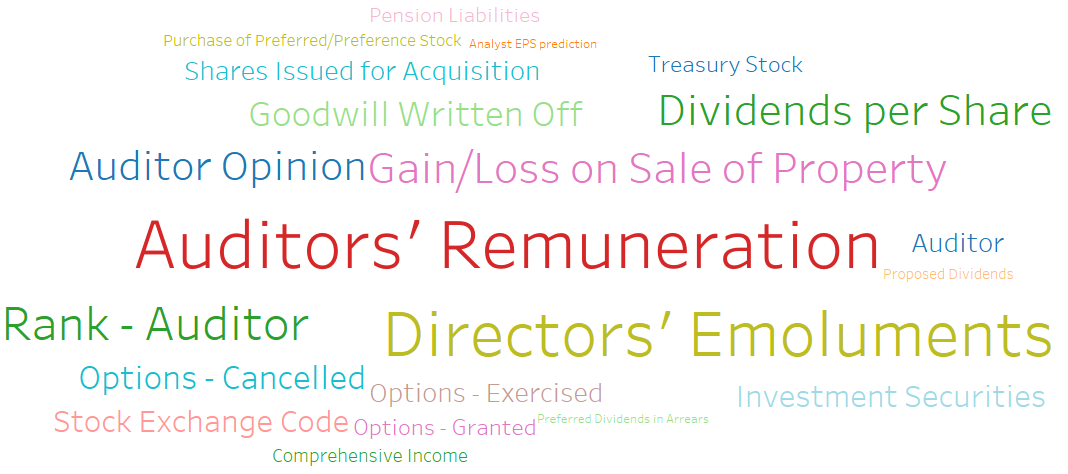
\includegraphics[width=1.0\linewidth]{v3_word_cloud_logistic_regression}
\caption{word cloud of features with greatest weight in our logistic regression model}
\end{figure}

\begin{figure}
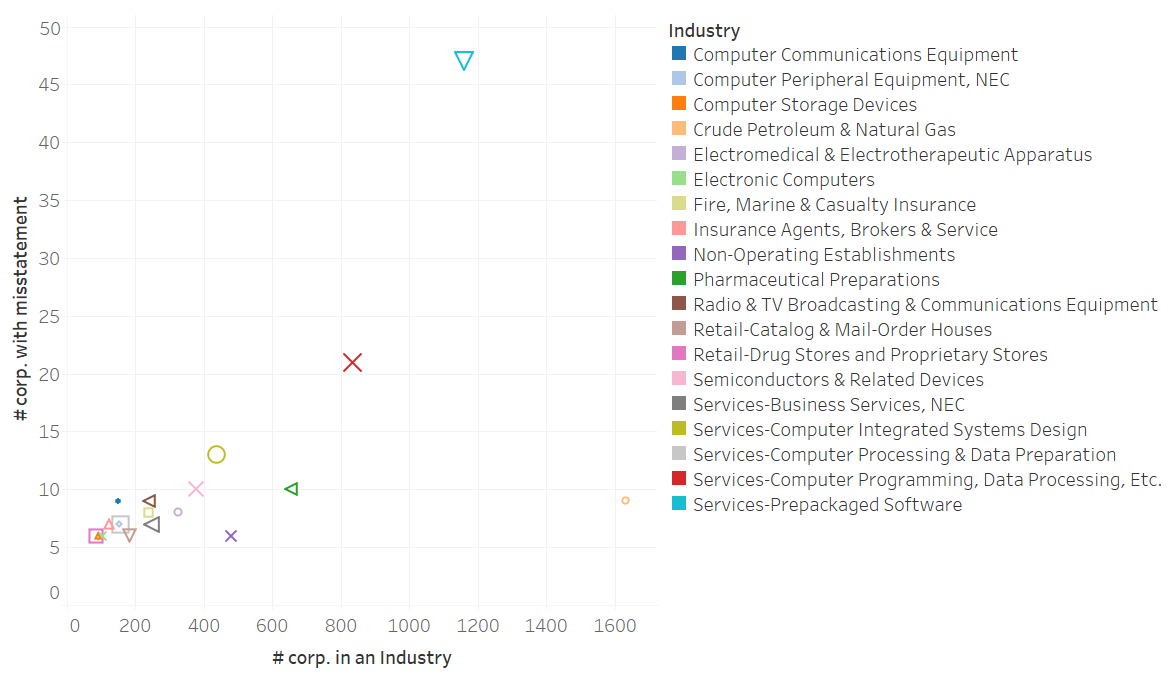
\includegraphics[width=1.0\linewidth]{num_corp_with_misstatements.png}
\caption{number of corporations with misstatements vs. total number of corporations in a given industry}
\end{figure} 


\end{column}
\begin{column}{\sepwid}\end{column} % Empty spacer column
\begin{column}{\onecolwid} % The third column

\begin{block}{Data Product} 
% What's your data product? Please demonstrate how it works.
Our data product is a program that takes in a set of financial statements as input and produces output labels as to whether these financial statements have been misstated or not.
\end{block}

\begin{block}{Lessons Learnt} 
% What did you learn from this project
\begin{itemize}
\item how to apply our machine learning and big data skills to financial datasets.
% \item We have learned how to clean, integrate and impute with real world datasets. 
\item Financial data is difficult to deal with. There are many fields and you need specialized knowledge. 
% \item learned accounting domain knowledge from Prof. Kim Trottier
\end{itemize}
\end{block}

\begin{alertblock}{Summary} 
% A high-level summary of your project. It should be self-contained and cover all the important aspects of your project.


\begin{itemize}
\item Detected misstatements correctly with accuracy of 82 \% using supervised machine learning algorithms.
\item Unsupervised learning algorithm partitioned the statements in two cluseters: misstatments and non-misstatements.
\item Analysed the most significant manipulations which include Auditors' remuneration,Emoluments,Earnings per share,etc.
\item Compared the difference between Actual EPS and Analyst predicted EPS for misstated corporations.
% \item 
% \begin{itemize}
% \item 
% \end{itemize}
\end{itemize}




\end{alertblock}

\begin{block}{References}
\nocite{*} % Insert publications even if they are not cited in the poster
\small{\bibliographystyle{unsrt}
\bibliography{sample}\vspace{0.75in}}
\end{block}

\begin{block}{Acknowledgements}
% \small{\rmfamily{Kim Trottier, Steven Bergner, Jiannan Wang, Hiral Patwa, Simranjit Singh Bhatia}} \\
\small{
\begin{itemize}
\item Kim Trottier, Associate Professor of Accounting, SFU
\item Steven Bergner, Research Associate, SFU
\item Jiannan Wang, Assistant Professor, SFU
\item Simranjit Singh Bhatia, TA
\item Hiral Patwa, TA
\end{itemize}
}
\end{block}


% \setbeamercolor{block alerted title}{fg=black,bg=norange} % Change the alert block title colors
% \setbeamercolor{block alerted body}{fg=black,bg=white} % Change the alert block body colors

% \begin{alertblock}{Contact Information}

% \begin{itemize}
% \item Web: \href{http://www.university.edu/smithlab}{http://www.university.edu/smithlab}
% \item Email: \href{mailto:john@smith.com}{john@smith.com}
% \item Phone: +1 (000) 111 1111
% \end{itemize}

% \end{alertblock}

% \begin{center}
% \begin{tabular}{ccc}
% 
\includegraphics[width=0.4\linewidth]{logo.png} & \hfill & 
\includegraphics[width=0.4\linewidth]{logo.png}
% \end{tabular}
% \end{center}

%----------------------------------------------------------------------------------------

\end{column} % End of the third column
\end{columns} % End of all the columns in the poster
\end{frame} % End of the enclosing frame
\end{document}
